\documentclass{article}

\usepackage[final]{style}
\usepackage[utf8]{inputenc}
\usepackage[T1]{fontenc}
\usepackage{amsmath, amssymb, amsfonts}
\usepackage{booktabs}
\usepackage{graphicx}
\usepackage{subcaption}
\usepackage{float}
\usepackage{microtype}
\usepackage{hyperref}
\hypersetup{hidelinks}

\title{STATS 305C Applied Statistics III\\Milestone 3: Model and Inference}
\author{Angikar Ghosal\\Stanford University \And Kaitlyn Wang\\Stanford University}
\date{}

\newcommand{\E}{\mathbb{E}}
\newcommand{\R}{\mathbb{R}}
\newcommand{\N}{\mathcal{N}}
\newcommand{\IW}{\mathcal{IW}}
\newcommand{\MN}{\mathcal{MN}}

\begin{document}
\maketitle
\vspace{-1.4em}
\small
\setlength{\parskip}{3pt}

\paragraph{Goal and data.}
Milestone 2 showed that web-quality filters agree on some broad axes but still
disagree substantially within topic. The main feedback was that a hierarchical
model should do something actionable, not only restate this fact. We therefore
fit a probabilistic model to six complete quality scores on a reproducible
120k-document sample from our 2.26M-document WebOrganizer subset, then use its
posterior predictions to propose data-selection mixes. The modeled scores are
DCLM, rounded FineWeb-Edu, and four perplexity-correlation filters
(ARC-Easy, PIQA, SciQ, LAMBADA). Bounded scores are clipped at $10^{-4}$ and
logit-transformed; FineWeb-Edu is treated as a continuous ordinal score. This is
a working likelihood rather than a perfect measurement model, but it lets us put
all filters on a common scale and fit a tractable multivariate model. All
responses and 17 heuristic covariates are standardized using the training split
only. We use 96,097 training documents and 23,903 held-out documents, with 24
topics, 24 formats, and the top 500 registered domains plus an ``other'' bucket.
QuRater is excluded from the main likelihood because it covers only 44 of the
100 sampled shards; we keep it for future validation rather than induce
missingness in the main model.

\begin{figure}[H]
  \centering
  \begin{subfigure}[t]{0.49\linewidth}
    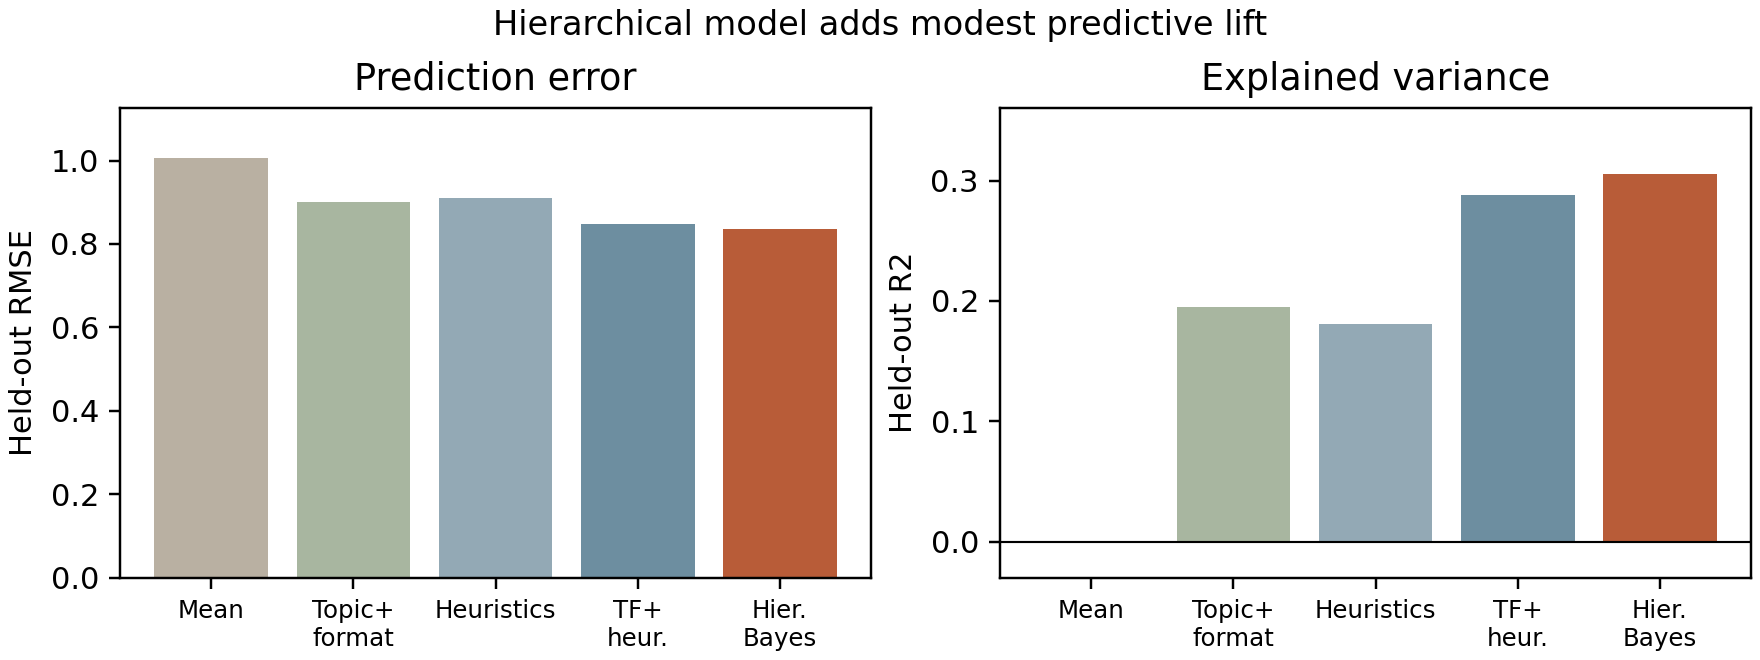
\includegraphics[width=\linewidth]{figures/week6_model_comparison.png}
    \caption{Held-out predictive comparison.}
  \end{subfigure}
  \hfill
  \begin{subfigure}[t]{0.49\linewidth}
    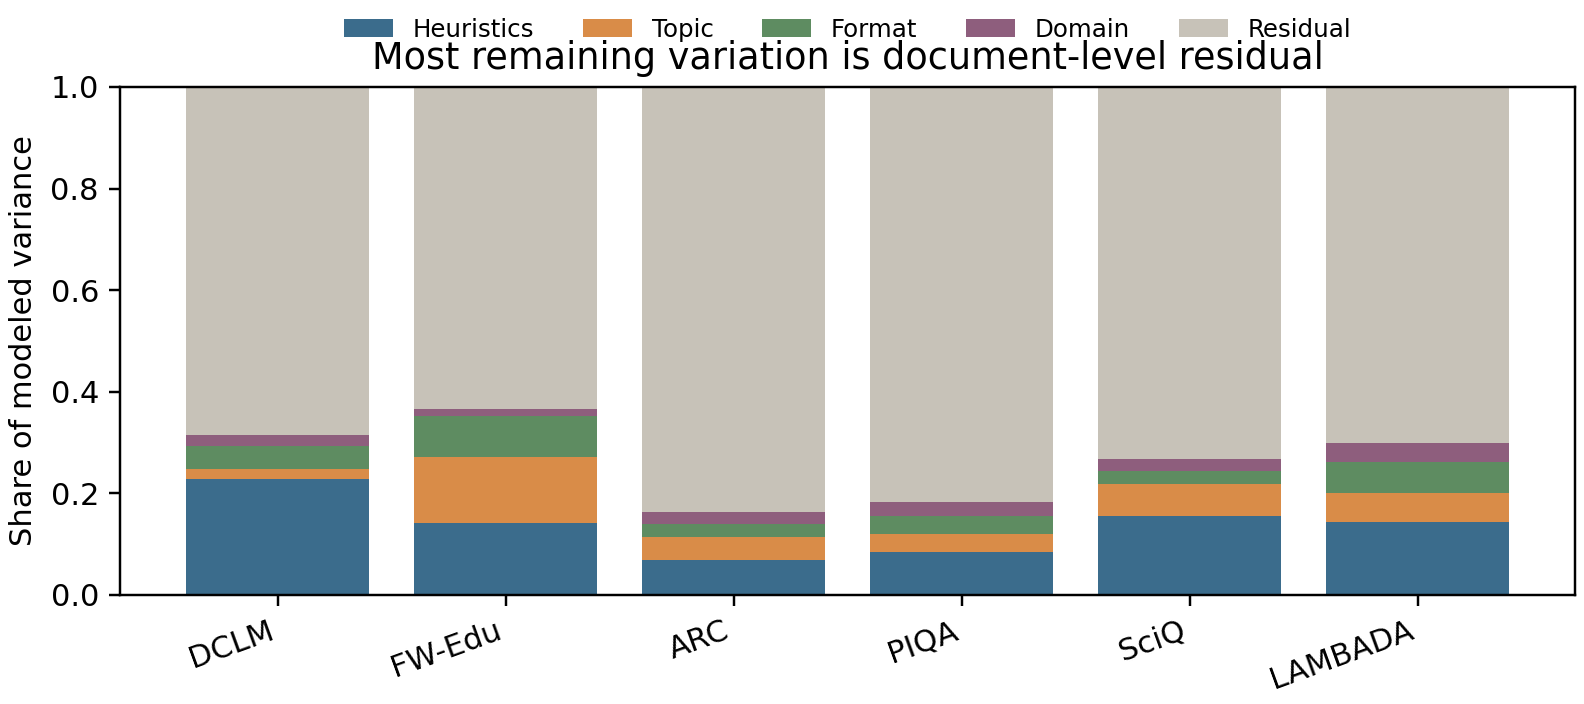
\includegraphics[width=\linewidth]{figures/week6_variance_decomposition.png}
    \caption{Posterior variance decomposition.}
  \end{subfigure}
  \vspace{-0.6em}
  \caption{The Bayesian hierarchy gives a modest but real predictive gain over
  fixed-effect baselines, and most unexplained variation remains document-level.}
  \label{fig:model}
\end{figure}

\paragraph{Generative model.}
For document $i$, let $y_i\in\R^6$ be the transformed standardized score vector
and $z_i$ be a design vector containing an intercept, standardized heuristics,
topic indicators, format indicators, and domain indicators. We fit the
multivariate Gaussian shrinkage model
\begin{align}
  y_i \mid B,\Sigma &\sim \N_6(z_i^\top B,\Sigma),\\
  B\mid\Sigma &\sim \MN_{p,6}(0,V_0,\Sigma),\\
  \Sigma &\sim \IW(\nu_0,S_0).
\end{align}
This is a hierarchical random-effects model in which topic, format, and domain
coefficients are partially pooled toward zero through block-specific prior
scales. We use prior standard deviations 10 for the intercept, 1.5 for
heuristics, 1 for topic and format effects, and 0.5 for domain effects; these
regularize the many sparse domain levels while leaving common topics/formats
flexible. The residual covariance $\Sigma$ is intentionally full rather than
diagonal because cross-filter disagreement is central to the scientific
question. We set $\nu_0=10$ and $S_0=I_6$. The prior mean is zero because the
responses are standardized; thus a positive coefficient directly means that the
covariate shifts a filter above its train-set average. The domain prior is
tighter than the topic/format priors because even the top-domain design contains
many sparse levels, and without shrinkage the model would overfit idiosyncratic
domain labels.

\paragraph{Inference.}
The model is conjugate, so we implemented a blocked Gibbs sampler. With
$Z$ the training design matrix and $Y$ the response matrix,
\[
  V_n=(Z^\top Z+V_0^{-1})^{-1},\qquad
  M_n=V_n Z^\top Y,
\]
and we alternate
\[
  B\mid\Sigma,Y \sim \MN(M_n,V_n,\Sigma),\quad
  \Sigma\mid B,Y \sim \IW(\nu_0+n+p,\ S_0+(Y-ZB)^\top(Y-ZB)+B^\top V_0^{-1}B).
\]
We ran 4 chains, 300 iterations each, discarded 150 burn-in iterations, and
kept every third draw, for 200 retained draws. Scalar diagnostics were stable:
the worst $\widehat R$ was 1.025 and the minimum approximate ESS was 143. For
prediction we use the posterior mean of $B$; for interpretation we summarize
posterior draws of $\Sigma$ and of the topic, format, domain, and heuristic
variance contributions. Baseline ridge penalties were selected by a validation
split inside the training set, so the held-out test set is used only once.

\paragraph{Posterior analysis and baselines.}
Figure~\ref{fig:model}a compares against simpler baselines. Mean prediction has
held-out RMSE 1.006 and $R^2\approx0$. Topic+format fixed effects reach
$R^2=0.195$, heuristics reach $R^2=0.181$, and topic+format+heuristics reach
$R^2=0.288$ with RMSE 0.847. The hierarchical model improves to RMSE 0.836 and
$R^2=0.305$. This is not a dramatic gain, but it is consistent across scores
and is largest for DCLM, FineWeb-Edu, SciQ, and LAMBADA. Figure~\ref{fig:model}b
shows why the problem remains hard: after observed covariates, residual
document-level variation explains roughly 63--84\% of each score's modeled
variance. Heuristics explain the largest non-residual share for DCLM (23\%),
SciQ (15\%), and LAMBADA (14\%); topic matters most for FineWeb-Edu (13\%).
The full residual covariance is useful: ARC-Easy and PIQA still have posterior
residual correlation 0.86 after covariates, while DCLM and LAMBADA retain only
0.18 correlation. Thus benchmark-specific filters share signal that is not
captured by topic, format, domain, or simple text heuristics. The result also
guards against overclaiming: the model beats the best baseline, but the
improvement is small, so most of the scientific value comes from uncertainty,
variance decomposition, and policy construction rather than raw prediction.

\begin{figure}[H]
  \centering
  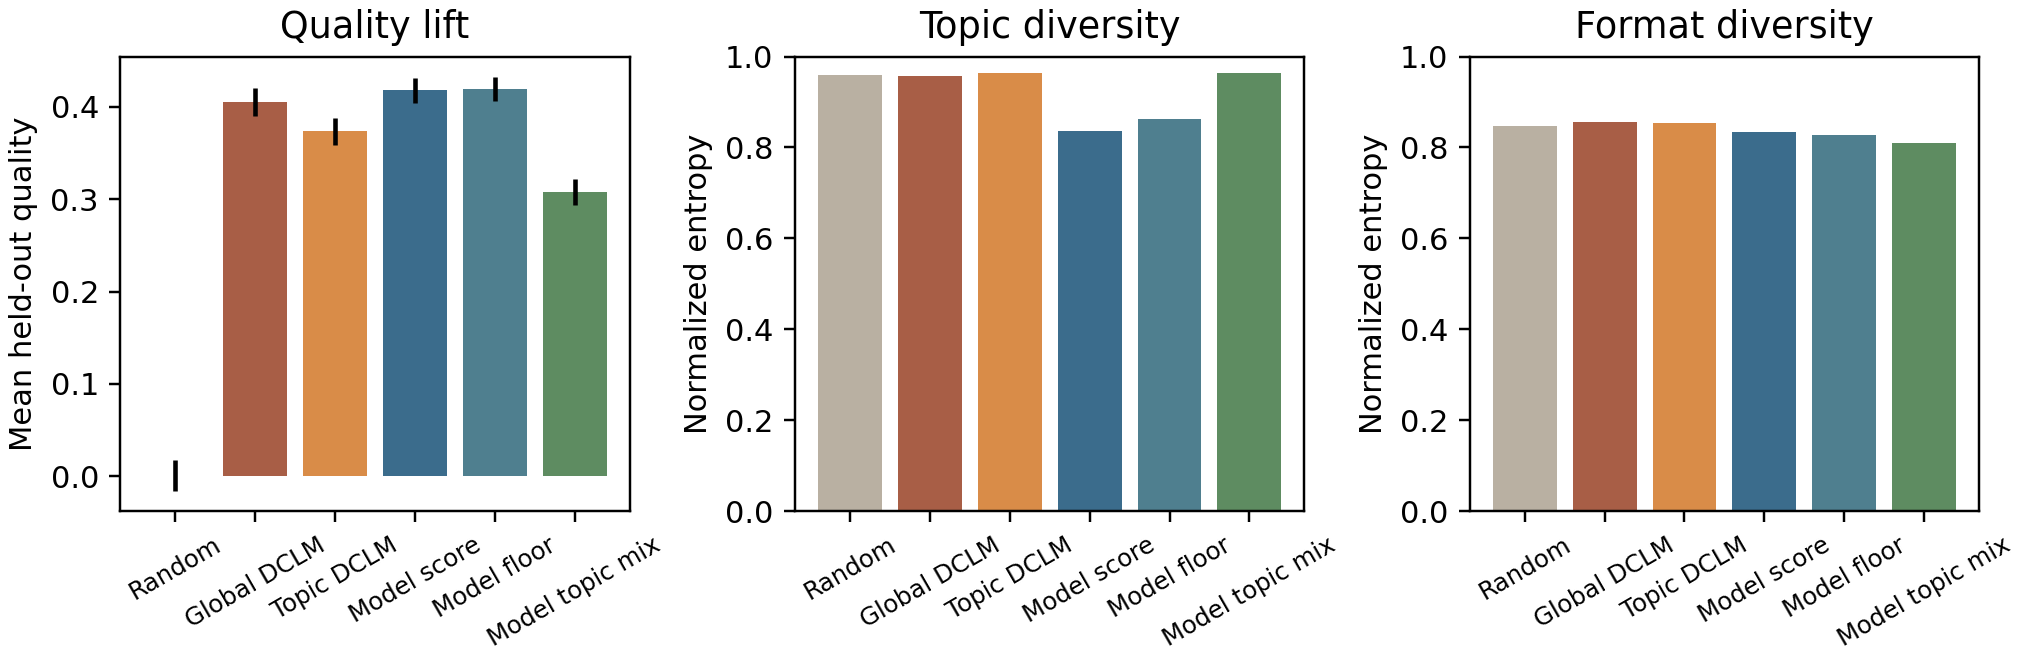
\includegraphics[width=\linewidth]{figures/week6_data_mix_comparison.png}
  \vspace{-1.0em}
  \caption{Actionable data-mix evaluation on held-out documents. All policies
  select the top 20\% except the random reference. The model-based policy gives
  the highest composite quality but trades off some diversity.}
  \label{fig:mix}
\end{figure}

\paragraph{Actionable data mix.}
We define composite held-out quality as the average of the six standardized
scores and compare top-20\% selection rules (Figure~\ref{fig:mix}). Random
selection has mean quality 0.001. A global DCLM threshold reaches 0.405 with
normalized topic entropy 0.957. A within-topic DCLM threshold preserves topic
entropy (0.964) but drops quality to 0.373. Ranking documents by posterior
predicted quality gives the best quality, 0.418, but lower topic entropy
(0.837). Our preferred actionable policy is a compromise: first keep a 5\%
within-topic floor by model score, then fill the remaining slots globally by
model score. It attains quality 0.419, covers all 24 topics, and improves topic
entropy to 0.862 relative to pure model ranking. The honest conclusion is that
the model adds a small predictive and selection advantage over DCLM, but the
gain comes with a diversity cost; a useful deployment should therefore expose
the quality-diversity frontier rather than choose a single global threshold.

\paragraph{Limitations and next steps.}
There are three important caveats. First, FineWeb-Edu is rounded ordinal, so a
cumulative-link submodel would be cleaner than the Gaussian working model.
Second, our evaluation uses held-out filter scores rather than downstream LM
training loss, so the data-mix result is a proxy for efficient pretraining, not
a direct demonstration. Third, QuRater's partial coverage prevents a fair
six-plus-four-filter joint model today. The next experiment should use the same
policy framework on a smaller corpus where tiny language models can actually be
trained from scratch, comparing DCLM, model-score, and model-with-topic-floor
mixtures at fixed token budgets.

\paragraph{AI assistance.}
We used Codex and Claude Code for implementation assistance, report drafting,
and debugging. The model, inference target, diagnostics, and interpretation were
checked against locally generated artifacts and code committed in the repository.

\end{document}
